\chapter{Probability, the Poisson Process, and Shot Noise}
\label{chap:e03}

\begin{chapteropening}
In the guided-tour chapter (\ref{chap:e00}) we already saw that what a telescope ultimately hands us is not a smooth electromagnetic wave but a string of discrete clicks: at some instant, in some pixel, on some channel, ``pop,'' one photon is recorded. In the previous chapter (\ref{chap:e02}) we then learned to characterize the ``wave'' side of this light with bandwidth and coherence time; but these waves are ultimately counted out one grain at a time by the detector. Since they are ``counted'' out, there must be fluctuation: the same star, the same telescope, and you count for ten milliseconds in a row, and the number of photons counted in each millisecond is almost never the same. This is not the instrument being broken, but the breathing that ``counting'' itself carries.

This chapter sets out to explain the ``language of counting'' thoroughly in one go. We first spend a few paragraphs reviewing the smallest set of words from probability theory (random variable, expectation, variance, independence), and then, starting from the extremely plain picture of ``slicing a stretch of time into many little cells,'' derive the Poisson distribution without skipping a step, and from it obtain the golden formula that runs through the whole book: the mean equals the variance, and the noise is proportional to $\sqrt{\mu}$. Finally we ask a deeper question: if one day you measure a variance that does not equal the mean, what does that mean? This ``what does it mean'' is precisely the entrance to the entire story that the later chapters devoted to second-order coherence $g^{(2)}$ will unfold.
\end{chapteropening}

\section{The Minimal Probability Review}
\label{sec:e03-review}

Before we start counting photons, we need four words. You have met them all in general physics and probability courses; here we nail them down with just ``a paragraph plus a formula'' each, so they can be called upon directly later.

\paragraph{Random variable.}
A random variable is simply ``one experiment will give a number, but you do not know in advance which number.'' The number of photons $N$ arriving in one millisecond is the most typical random variable: it can only take non-negative integers $0,1,2,\dots$, and each value corresponds to a probability. To describe a (discrete) random variable is to give the probability $P(N)$ of it taking each value, satisfying
\begin{equation}
  P(N)\ge 0,\qquad \sum_{N=0}^{\infty}P(N)=1 .
  \label{eq:e03-normalization}
\end{equation}
\begin{formulaexplain}
$N$ is the integer count obtained in one measurement; $P(N)$ is the probability that ``this time exactly $N$ are counted.'' The first equation says probabilities are non-negative, the second says that adding up the probabilities of all possible cases must equal $1$: something has to happen.
\end{formulaexplain}
Here $N$ is a dimensionless integer (just ``how many''), and $P(N)$ is also a dimensionless pure number, taking values between $0$ and $1$. The second condition of Eq.~\eqref{eq:e03-normalization} is called normalization, and it is the ``conservation law'' that all later derivations must satisfy self-consistently: no matter how complicated a form we write the distribution in, summing $N$ from $0$ to infinity, the answer must return to $1$.

\paragraph{Expectation.}
The expectation is the ``mean value,'' but it is a theoretical, weighted mean: multiply each possible value $N$ by its probability and sum. We use angle brackets $\langle\cdot\rangle$ to denote taking the expectation,
\begin{equation}
  \langle N\rangle=\sum_{N=0}^{\infty}N\,P(N).
  \label{eq:e03-expectation}
\end{equation}
\begin{formulaexplain}
$\langle N\rangle$ is read as ``the expectation of $N$'' or ``the mean of $N$''; it weights each possible count $N$ by its probability of occurrence $P(N)$ and sums. It is not the result of any one measurement, but the average destination after infinitely many repetitions.
\end{formulaexplain}
Note that $\langle N\rangle$ is generally not an integer: an average of $100.3$ photons per millisecond is perfectly reasonable, even though any single time you can only count an integer. The expectation is additive: for any two random variables $X,Y$, $\langle X+Y\rangle=\langle X\rangle+\langle Y\rangle$, whether or not they are independent. This property that ``the expectation is always additive'' will be used repeatedly later when assembling the little cells.

\paragraph{Variance.}
Having only the mean is not enough; we also want to know ``how far each result is from the mean.'' The variance measures precisely the size of the fluctuation: take the deviation $N-\langle N\rangle$, square it (so that positive and negative deviations both become positive contributions), then take the expectation,
\begin{equation}
  \operatorname{Var}(N)=\big\langle (N-\langle N\rangle)^2\big\rangle
  =\langle N^2\rangle-\langle N\rangle^2 .
  \label{eq:e03-variance}
\end{equation}
\begin{formulaexplain}
$\operatorname{Var}(N)$ is the variance, measuring the spread of the counts about their mean; it equals ``the mean of the square'' minus ``the square of the mean.'' The larger it is, the more each counted result ``drifts.''
\end{formulaexplain}
The second equality of Eq.~\eqref{eq:e03-variance} is an identity, obtained by expanding the definition: $\langle(N-\langle N\rangle)^2\rangle=\langle N^2-2N\langle N\rangle+\langle N\rangle^2\rangle=\langle N^2\rangle-2\langle N\rangle\langle N\rangle+\langle N\rangle^2=\langle N^2\rangle-\langle N\rangle^2$, using here that the expectation is additive and that ``the expectation of a constant is itself.'' The dimension of the variance is the square of the dimension of $N$ (here $N$ is dimensionless, so the variance is dimensionless too). Its square root
\[
  \sigma=\sqrt{\operatorname{Var}(N)}
\]
is called the standard deviation, with the same unit as $N$, and is what we everyday call ``how long the error bar is.'' Remember this intuition: $\sigma$ is the ``fluctuation scale'' comparable to $N$, and the variance is its square.

\paragraph{Independence.}
Two random variables being independent means, intuitively, ``knowing the result of one is of no help whatsoever to the probability distribution of the other.'' In formula terms, the joint probability factors into the product of the individual probabilities: $P(X=x,\,Y=y)=P(X=x)\,P(Y=y)$. Independence gives us an extremely useful gift, the variance is additive:
\begin{equation}
  \operatorname{Var}(X+Y)=\operatorname{Var}(X)+\operatorname{Var}(Y)
  \quad(\text{when }X,Y\text{ are independent}).
  \label{eq:e03-var-additive}
\end{equation}
\begin{formulaexplain}
Only when $X$ and $Y$ are mutually independent does the variance of their sum equal the sum of their individual variances. This ``independent implies additive variance'' is the key lever later for assembling many little cells into one big bin and thereby computing the shot noise.
\end{formulaexplain}
Compare: the additivity of the expectation $\langle X+Y\rangle=\langle X\rangle+\langle Y\rangle$ is unconditional, whereas the additivity of the variance \eqref{eq:e03-var-additive} requires independence as a premise. The reason hides in the cross term: $\operatorname{Var}(X+Y)=\operatorname{Var}(X)+\operatorname{Var}(Y)+2\operatorname{Cov}(X,Y)$, where the covariance $\operatorname{Cov}(X,Y)=\langle XY\rangle-\langle X\rangle\langle Y\rangle$ measures the correlation of the two; when independent, $\langle XY\rangle=\langle X\rangle\langle Y\rangle$, the covariance goes to zero, and only then do the variances add cleanly. Please remember this sentence well, because the whole suspense of ``what does it mean when the variance does not equal the mean'' at the chapter's end hides in whether this covariance is zero.

With these four words in hand, we can begin to really count photons.

\section{The Mean Count in One Time Bin}
\label{sec:e03-mean}

Back in front of the telescope. In the previous chapter, the detector turned light into a string of discrete clicks. Now we do the plainest thing: choose a time window (time bin) of width denoted $\Delta t$, then count how many photons fall into this window.

If the mean photon arrival rate of this light is $R_\gamma$, then the mean count in one bin is the rate times the time:
\begin{equation}
  \mu=R_\gamma\,\Delta t .
  \label{eq:e03-mean-count}
\end{equation}
\begin{formulaexplain}
$\mu$ is the mean number of photons in one time bin (i.e.\ $\langle N\rangle$); $R_\gamma$ is the mean arrival rate, in units of $\mathrm{s^{-1}}$; $\Delta t$ is the bin width, in units of $\mathrm{s}$. Multiplying the two, the seconds cancel, and $\mu$ is the dimensionless ``how many on average.''
\end{formulaexplain}
Let us make the units and orders of magnitude concrete. The dimension of $R_\gamma$ is ``how many per second,'' i.e.\ $\mathrm{s^{-1}}$; the dimension of $\Delta t$ is the second $\mathrm{s}$; multiplying the two, the second and the ``per second'' cancel, and $\mu$ is a pure number. Take a real set of optical observation numbers: a star of moderate brightness, a metre-class telescope, a narrow-band channel, with a detected photon rate of about $R_\gamma=10^{5}\,\mathrm{s^{-1}}$; if we slice time into bins of $\Delta t=1\,\mathrm{ms}=10^{-3}\,\mathrm{s}$, then
\[
  \mu=R_\gamma\,\Delta t=10^{5}\,\mathrm{s^{-1}}\times10^{-3}\,\mathrm{s}=100 .
\]
That is, on average about $100$ photons fall in per millisecond.

Here the two words ``on average'' must be broken down and chewed through, because they are the fulcrum of everything in this chapter. Equation~\eqref{eq:e03-mean-count} absolutely does not say ``every $1\,\mathrm{ms}$ window receives exactly $100$ photons.'' It says: if you take, under completely identical conditions (the star equally bright, the telescope equally large, the efficiency equally high), thousands upon thousands of $1\,\mathrm{ms}$ windows, add up the photons counted in each window, and divide by the number of windows, this ``measured mean'' will approach $100$. In the real event stream, this one bin might be $92$, the next $107$, the next $100$: they breathe up and down around $100$. $\mu$ is the centre line of this breathing, not the measured value of any single time.

The crux is: even if you freeze all external conditions, holding the star, atmosphere, telescope, and detector perfectly still, this breathing does not go away. This is not ``uncertain instrumental noise'' but the statistical fluctuation that the very act of ``counting discrete things'' carries. To understand what law this fluctuation obeys and how large it is, we need to equip the physical intuition ``photons arrive sparsely and independently of one another'' with a set of mathematics, and that is the Poisson distribution.

\section{From the Binomial to the Poisson Distribution: A Derivation Skipping No Step}
\label{sec:e03-poisson}

\paragraph{Slicing the bin into many little cells}

The question we want to answer is: given that the mean value is $\mu$, what exactly does the probability $P(N)$ of ``counting exactly $N$'' look like?

First set up a physical assumption, the soul of the entire Poisson picture: given the mean rate, photons arrive independently and without memory of one another. By ``without memory'' we mean that the previous photon having just arrived neither summons the next one to hurry along too (that would be bunching) nor warns the next one to stay away (that would be antibunching); whether a photon appears in each extremely short stretch of time is determined only by the length of that stretch, and has nothing to do with what happened elsewhere. This is the simplest arrival pattern behind the ``on average'' of the previous section. This chapter first assumes it holds and computes the conclusion to the end; as for when it is broken, we leave that for the final section to point out.

With this assumption, we can compute using a very concrete picture. Slice the time bin of width $\Delta t$ uniformly into $M$ very short little cells, each of width
\[
  \delta t=\frac{\Delta t}{M}.
\]
As long as $M$ is large enough and $\delta t$ short enough, each little cell can hold at most one photon: the probability of two photons squeezing into the same extremely short cell at once is negligible. So each little cell degenerates into the simplest ``coin flip'': either a click (a photon appears) or nothing. The probability that a little cell registers a click is approximately
\begin{equation}
  p=R_\gamma\,\delta t .
  \label{eq:e03-cell-prob}
\end{equation}
\begin{formulaexplain}
$p$ is the probability of one click appearing in a single little cell; $R_\gamma$ is the arrival rate; $\delta t$ is the cell width. The higher the rate and the longer the cell, the greater the chance of catching a photon in this cell, but as long as $\delta t$ is short enough, $p$ is a very small number.
\end{formulaexplain}
$p$ is a dimensionless probability ($\mathrm{s^{-1}}\times\mathrm{s}$ cancels to a pure number). Note there is a self-consistency check here: the mean number of clicks over all little cells, added up, should be exactly the mean count of the whole bin. Indeed, $M$ little cells, each contributing $p$ on average, gives a total mean of
\[
  M\,p=M\cdot R_\gamma\frac{\Delta t}{M}=R_\gamma\,\Delta t=\mu .
\]
This $Mp=\mu$ is the only quantity we must ``nail fixed'' when taking the limit next: no matter how finely we slice the cells ($M\to\infty$, $p\to0$), the product $Mp$ always equals $\mu$.

\paragraph{First write down the binomial distribution}

Now counting photons becomes a pure combinatorics problem: what is the probability that ``among $M$ little cells, exactly $N$ cells registered a click''? Since the cells are mutually independent, each specific case of ``which $N$ cells click and the other $M-N$ do not'' has probability $p^{N}(1-p)^{M-N}$; and ``choosing which $N$ of the $M$ cells click'' has $\binom{M}{N}$ ways in total. Multiplying the number of ways by the probability of each case gives the binomial distribution:
\begin{equation}
  P_M(N)=\binom{M}{N}p^{N}(1-p)^{M-N},
  \qquad \binom{M}{N}=\frac{M!}{N!\,(M-N)!}.
  \label{eq:e03-binomial}
\end{equation}
\begin{formulaexplain}
$P_M(N)$ is the probability of exactly $N$ cells clicking after slicing the bin into $M$ little cells. $p^{N}$ is these $N$ cells all clicking, $(1-p)^{M-N}$ is the rest not clicking, and $\binom{M}{N}$ is the number of ways to ``choose which $N$ cells.'' Multiplying the three gives the result.
\end{formulaexplain}
This equation contains no approximation yet; it is an exact translation of the little-cell picture into a probability. $\binom{M}{N}$ is read ``$M$ choose $N$,'' the binomial coefficient; $N!$ ($N$ factorial) is the normalization factor of the number of permutations, responsible for dividing out the repetitions of ``the same few cells, only counted in a different order.'' What we do next is to let the cells become infinitely fine: $M\to\infty$, $p\to0$, while pressing down hard on $Mp=\mu$. We split Eq.~\eqref{eq:e03-binomial} into three pieces ($\binom{M}{N}$, $p^N$, $(1-p)^{M-N}$) and take the limit piece by piece.

\paragraph{\texorpdfstring{Step one: $\binom{M}{N}p^{N}\to \mu^{N}/N!$}{Step one: the limit of the binomial-coefficient term}}

Substitute $p=\mu/M$ (this is a rewriting of $Mp=\mu$), and first merge the binomial coefficient with $p^N$:
\[
  \binom{M}{N}p^{N}
  =\frac{M!}{N!\,(M-N)!}\left(\frac{\mu}{M}\right)^{N}
  =\frac{1}{N!}\cdot\frac{M!}{(M-N)!}\cdot\frac{\mu^{N}}{M^{N}} .
\]
The middle piece $\dfrac{M!}{(M-N)!}$ is in fact a product of $N$ consecutive descending factors:
\[
  \frac{M!}{(M-N)!}=M(M-1)(M-2)\cdots(M-N+1) .
\]
It has $N$ factors in all, each approximately equal to $M$ (because $N$ is a fixed finite integer while $M$ tends to infinity, so the differences of $M-1,M-2,\dots$ from $M$ are negligible). More precisely, divide it by $M^{N}$:
\[
  \frac{M(M-1)\cdots(M-N+1)}{M^{N}}
  =1\cdot\Big(1-\tfrac{1}{M}\Big)\Big(1-\tfrac{2}{M}\Big)\cdots\Big(1-\tfrac{N-1}{M}\Big)
  \xrightarrow[M\to\infty]{}1 .
\]
Each parenthesis tends to $1$ as $M\to\infty$, and there are only a fixed $N-1$ parentheses, so the whole product tends to $1$. So the limit of the first piece is clean and neat:
\begin{equation}
  \binom{M}{N}p^{N}
  =\frac{\mu^{N}}{N!}\cdot\frac{M(M-1)\cdots(M-N+1)}{M^{N}}
  \xrightarrow[M\to\infty]{}\frac{\mu^{N}}{N!}.
  \label{eq:e03-limit-first}
\end{equation}
\begin{formulaexplain}
After substituting $p=\mu/M$, the binomial coefficient merges with $p^N$; the $N$ descending factors in the numerator, divided by $M^N$, tend to $1$ one by one, leaving only $\mu^N/N!$. This step turns the ``combinatorial count of choosing cells'' into the familiar $\mu^N/N!$ of the Poisson formula.
\end{formulaexplain}

\paragraph{\texorpdfstring{Step two: $(1-p)^{M}\to e^{-\mu}$}{Step two: the limit of the no-click probability}}

Now handle the third piece $(1-p)^{M-N}$. Substituting $p=\mu/M$ likewise:
\[
  (1-p)^{M-N}=\Big(1-\frac{\mu}{M}\Big)^{M-N}
  =\Big(1-\frac{\mu}{M}\Big)^{M}\cdot\Big(1-\frac{\mu}{M}\Big)^{-N}.
\]
First look at the second factor $\big(1-\mu/M\big)^{-N}$: the exponent $-N$ is a fixed finite number, while the base $1-\mu/M\to 1$, so this factor tends to $1^{-N}=1$ and can be discarded. What really matters is the first factor $\big(1-\mu/M\big)^{M}$. Here we call upon a standard limit by name, the general form of the definition of the natural constant $e$:
\begin{equation}
  \lim_{M\to\infty}\Big(1-\frac{\mu}{M}\Big)^{M}=e^{-\mu}.
  \label{eq:e03-elimit}
\end{equation}
\begin{formulaexplain}
This is a known standard limit (the definition of $e$): $\big(1+x/M\big)^{M}\to e^{x}$, taking $x=-\mu$ gives $e^{-\mu}$. It condenses the joint probability of ``many little cells all not clicking'' into a single exponential factor.
\end{formulaexplain}
Why does \eqref{eq:e03-elimit} hold, rather than being an incantation? We can verify it by taking the logarithm, using the Taylor expansion of the logarithm $\ln(1+u)=u-\tfrac12u^{2}+\cdots$ (when $u$ is small):
\[
  \ln\Big(1-\frac{\mu}{M}\Big)^{M}
  =M\ln\Big(1-\frac{\mu}{M}\Big)
  =M\left(-\frac{\mu}{M}-\frac{\mu^{2}}{2M^{2}}-\cdots\right)
  =-\mu-\frac{\mu^{2}}{2M}-\cdots .
\]
As $M\to\infty$, all terms except the first, which contain $1/M$, vanish, leaving only $-\mu$; taking the exponential to restore gives $e^{-\mu}$. Physically, this $e^{-\mu}$ is precisely the condensation of the total probability that ``a great many little cells each register exactly no click'': $M$ little cells, each with no-click probability $1-p$, all not clicking is $(1-p)^{M}$, which in the limit becomes $e^{-\mu}$.

\paragraph{Putting it together: the Poisson distribution}

Multiplying the two limits \eqref{eq:e03-limit-first} and \eqref{eq:e03-elimit} (the discarded $\big(1-\mu/M\big)^{-N}\to1$ from the second piece already merged in), the binomial distribution \eqref{eq:e03-binomial} converges to the Poisson distribution:
\begin{equation}
  P(N)=\lim_{M\to\infty}P_M(N)
  =e^{-\mu}\,\frac{\mu^{N}}{N!}.
  \label{eq:e03-poisson}
\end{equation}
\begin{formulaexplain}
$P(N)$ is the probability of counting exactly $N$ photons in one bin when the mean count is $\mu$. $e^{-\mu}$ comes from ``many little cells not clicking,'' $\mu^{N}$ is the weight that the larger the mean the more it favours high counts, and $N!$ removes the repetition of the ordering of the clicks. This is the counting law of sparse independent arrival.
\end{formulaexplain}
Each part of this equation has a corresponding intuition. The exponential factor $e^{-\mu}$ is the ``background base note,'' representing the contribution of the great many empty little cells, the larger $\mu$ the lower it presses; $\mu^{N}$ is the ``the brighter the more skewed toward many'' climbing term; $N!$ is the combinatorial normalization, smoothing away the irrelevant ordering of who clicks first among the $N$ clicks. We can do a normalization self-check on the spot, using the Taylor series of the exponential function $\sum_{N=0}^{\infty}\mu^{N}/N!=e^{\mu}$ (this is the standard expansion of $e^{\mu}$):
\[
  \sum_{N=0}^{\infty}P(N)
  =e^{-\mu}\sum_{N=0}^{\infty}\frac{\mu^{N}}{N!}
  =e^{-\mu}\cdot e^{\mu}=1 .
\]
Just as Eq.~\eqref{eq:e03-normalization} requires, the total probability returns to $1$, showing that we did not lose or overcount any probability while taking the limit.

Let us also verify the expectation on the spot, to confirm that this $\mu$ is indeed the mean count (and not some coincidentally same-named letter). By definition \eqref{eq:e03-expectation},
\[
  \langle N\rangle
  =\sum_{N=0}^{\infty}N\,e^{-\mu}\frac{\mu^{N}}{N!}
  =e^{-\mu}\sum_{N=1}^{\infty}\frac{\mu^{N}}{(N-1)!}
  =e^{-\mu}\,\mu\sum_{N=1}^{\infty}\frac{\mu^{N-1}}{(N-1)!}
  =e^{-\mu}\,\mu\,e^{\mu}=\mu .
\]
The first step drops the $N=0$ term (which contributes zero) and sums from $N=1$; the second uses $N/N!=1/(N-1)!$ to cancel one factor; the third changes the variable to $k=N-1$, and that sum is again $e^{\mu}$. The result $\langle N\rangle=\mu$, complete. At this point the Poisson distribution lives up to its name: its mean count is precisely $\mu=R_\gamma\Delta t$.

One sentence worth stressing, lest the reader misunderstand the Poisson distribution as some ``mysterious randomness'': it describes absolutely not ``causeless chaos,'' but on the contrary the most orderly, most even-tempered kind of arrival: a string of sparse independent clicks with no extra memory, not summoning one another and not avoiding one another. Precisely because it is so ``standard,'' it becomes the baseline against which all deviations are measured.

\section{Shot Noise: The Variance Equals the Mean}
\label{sec:e03-shotnoise}

\paragraph{Computing the variance from the independent superposition of little cells}

Having the distribution, next we measure the fluctuation. We want to prove that the variance of the Poisson count is exactly equal to its mean. The least laborious and most physically flavoured method is still to return to the little-cell picture, using the lever ``independent implies additive variance'' prepared in the first section.

Give the $i$-th little cell an indicator variable $X_i$: if this cell clicks, $X_i=1$; if not, $X_i=0$. The total count is the sum over all little cells, $N=\sum_{i=1}^{M}X_i$. Each $X_i$ takes only $0$ or $1$, the simplest Bernoulli variable, whose mean and variance are easy to compute:
\[
  \langle X_i\rangle=1\cdot p+0\cdot(1-p)=p,\qquad
  \langle X_i^{2}\rangle=1^{2}\cdot p+0^{2}\cdot(1-p)=p ,
\]
so by the variance definition \eqref{eq:e03-variance},
\[
  \operatorname{Var}(X_i)=\langle X_i^{2}\rangle-\langle X_i\rangle^{2}=p-p^{2}=p(1-p).
\]
Now invoke the assumption: different little cells are mutually independent, so the variance is additive (Eq.~\eqref{eq:e03-var-additive}); adding up the $M$ identical little cells,
\[
  \operatorname{Var}(N)=\sum_{i=1}^{M}\operatorname{Var}(X_i)=M\,p(1-p)=Mp\,(1-p)=\mu\,(1-p).
\]
The last step used $Mp=\mu$. Now take the limit of infinitely fine cells $p=\mu/M\to0$, that $(1-p)$ tends to $1$, and what remains is precisely
\begin{equation}
  \operatorname{Var}(N)=\mu .
  \label{eq:e03-var-equals-mean}
\end{equation}
\begin{formulaexplain}
The variance of the Poisson count is exactly equal to its mean $\mu$. It comes from the superposition of ``$M$ independent little cells, each contributing a variance of $p(1-p)$,'' and in the fine-slicing limit $(1-p)\to1$, the total variance converges to $\mu$. Mean equal to variance is the fingerprint of Poisson statistics.
\end{formulaexplain}
Please appreciate how slender and powerful this $\operatorname{Var}(N)=\mu$ is: it says that for independently arriving photons, you need not measure anything extra: knowing only the mean count $\mu$, you automatically know the size of the fluctuation. Mean and variance are not two independent quantities, but are locked into the same number by the assumption of ``independent arrival.'' This also explains why it is called shot noise: like raindrops smacking a tin roof, the noise is not the roof being broken, but the raindrops themselves arriving discretely one grain at a time, the graininess naturally bringing fluctuation.

\paragraph{Relative noise, signal-to-noise ratio, and order of magnitude}

Having the variance, the standard deviation is its square root:
\begin{equation}
  \sigma=\sqrt{\operatorname{Var}(N)}=\sqrt{\mu}.
  \label{eq:e03-sigma}
\end{equation}
\begin{formulaexplain}
$\sigma$ is the standard deviation of the count, i.e.\ the length of the error bar, equal to $\sqrt{\mu}$. The absolute fluctuation grows with the mean count, but grows more slowly than the mean (only as the square root).
\end{formulaexplain}
Note that $\sigma=\sqrt{\mu}$ has the same dimension as $N$, both ``how many,'' and can be drawn directly as an error bar on the count: a bin with a mean of $100$ counts has a typical fluctuation of about $\sqrt{100}=10$ (see Figure~\ref{fig:e03-poisson}; that distribution spreading around $\mu$ and the fluctuation band of $\pm\sqrt{\mu}$ are the very look of this statistics). The absolute fluctuation does rise with brightness, but what really determines the quality of the measurement is how large it is relative to the signal itself. So we define the relative shot noise
\begin{equation}
  \frac{\sigma}{\mu}=\frac{\sqrt{\mu}}{\mu}=\frac{1}{\sqrt{\mu}} .
  \label{eq:e03-relative}
\end{equation}
\begin{formulaexplain}
The relative fluctuation equals $1/\sqrt{\mu}$: the more you count, the smaller the relative noise, but it improves only slowly as the square root. To halve the relative error, you must count four times as many photons.
\end{formulaexplain}
This $1/\sqrt{\mu}$ is the most oft-recited line in astronomical observation, and translating it into orders of magnitude is especially satisfying. Its reciprocal, $\mu$ against its own fluctuation, is precisely the signal-to-noise ratio (SNR):
\begin{equation}
  \mathrm{SNR}=\frac{\text{signal}}{\text{noise}}=\frac{\mu}{\sigma}=\frac{\mu}{\sqrt{\mu}}=\sqrt{\mu}.
  \label{eq:e03-snr}
\end{equation}
\begin{formulaexplain}
When pure shot noise dominates, the signal-to-noise ratio equals $\sqrt{\mu}$: divide the signal $\mu$ by its fluctuation $\sqrt{\mu}$. The more photons accumulated, the higher the signal-to-noise ratio, likewise growing as the square root.
\end{formulaexplain}
Let us put in real numbers to feel how ``expensive'' this square-root law is. If one stretch of integration accumulates on average $\mu=10^{4}$ photons, then the relative noise is $1/\sqrt{10^4}=1/100=1\%$ and the signal-to-noise ratio is $\sqrt{10^4}=100$, a rather beautiful measurement. Conversely, if in an extremely faint source, an extremely short bin, there is on average only $\mu=1$ photon, then the relative noise is $1/\sqrt{1}=100\%$ and the signal-to-noise ratio is only $1$: here the discrete count itself is the dominant noise, whether you count $0$ or $2$ is almost a coin flip, and any fine physical quantity is drowned in the raw fluctuation of ``whether there is a photon or not.''

This square-root law also incidentally explains the sense of ``twice the effort for half the result'' fatalism in astronomical observation: to press the relative error from $1\%$ further down to $0.5\%$, $\mu$ must rise from $10^4$ to $4\times10^4$: the integration time must quadruple to buy a halving of the error. Shot noise is the floor of all more complicated error budgets; later, no matter whether we add in background, dead time, or the source's own variation, we must first stand on this floor of $\sqrt{\mu}$ and build up from there.

\begin{figure}[tbp]
\centering
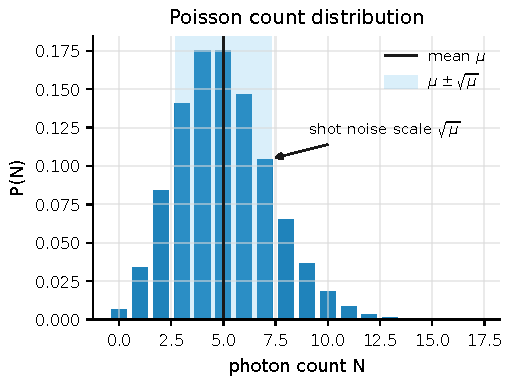
\includegraphics[width=0.85\linewidth]{figures/generated/chapter_01/ch01_photon_count_statistics.pdf}
\caption{The basic shape of the Poisson count distribution (here taking a single mean count $\mu$ as illustration). When the mean count is $\mu$, the distribution spreads around $\mu$, the variance also equals $\mu$, so the scale of the fluctuation (the error bar) is $\sqrt{\mu}$, and the relative shot noise is $1/\sqrt{\mu}$. The figure marks the mean line and the $\pm\sqrt{\mu}$ fluctuation band.}
\label{fig:e03-poisson}
\end{figure}

\section{When the Variance No Longer Equals the Mean: A Question Left for Later}
\label{sec:e03-beyond}

Now let us look at the whole chapter's logic in reverse. We obtained $\operatorname{Var}(N)=\mu$ by relying on a very hard premise: that arrivals in different little cells are mutually independent, so that the variance is additive (Eq.~\eqref{eq:e03-var-additive}). Once this premise holds, mean and variance are locked into the same number. So, conversely: if one day in an experiment you carefully measure the variance and the mean and find that they are not equal, then this chain must have broken at the link of ``independence.''

So ``whether the variance is larger or smaller than the mean'' becomes a probe reading directly the behaviour of the photons. Let us define a convenient ratio, the Mandel $Q$ parameter, to quantify the deviation:
\begin{equation}
  Q=\frac{\operatorname{Var}(N)-\mu}{\mu}.
  \label{eq:e03-mandelQ}
\end{equation}
\begin{formulaexplain}
$Q$ measures the deviation of the counting statistics from Poisson: $Q=0$ is Poisson (independent arrival); $Q>0$ the variance exceeds the mean, called super-Poisson; $Q<0$ the variance is less than the mean, called sub-Poisson. It translates ``independent or not'' into a measurable number.
\end{formulaexplain}
The three cases correspond to three utterly different physical pictures. $Q=0$, the variance equals the mean, is the Poisson baseline of this chapter, the photons not greeting one another. $Q>0$, the variance bulges out, is called super-Poissonian: the photons tend to arrive in clumps, one arrives and its companions are more likely to come in company too, as though they love to huddle: this is bunching, the hallmark of thermal light and starlight, kinds of chaotic light. $Q<0$, the variance is pressed down, is called sub-Poissonian: the photons push one another away, one has just arrived and the next deliberately hides and stays away, arriving even more ``evenly'' than random: this is antibunching, the fingerprint of genuinely non-classical light such as single-photon sources, which a classical electromagnetic wave can never produce no matter how it is manipulated.

Pushing these two pictures to the extreme, we touch the covariance planted at the chapter's end: bunching means the arrivals at neighbouring times are positively correlated ($\operatorname{Cov}>0$, the variance pushed up), and antibunching means negatively correlated ($\operatorname{Cov}<0$, the variance whittled down). Measuring this correlation strength of ``after one photon arrives, whether another photon is more or less likely to follow closely'' requires a dedicated tool: the second-order coherence function $g^{(2)}(\tau)$. What it measures is precisely the relative probability that ``given that a photon is detected at time $t$, another photon is detected again after a further $\tau$'': $g^{(2)}(0)>1$ is bunching, $g^{(2)}(0)<1$ is antibunching, and $g^{(2)}=1$ returns to the everywhere-independent Poisson baseline of this chapter.

In other words, this chapter has spoken the ``language of counting'' to its very boundary: as long as photons arrive independently, everything is locked down by the two equations $\mu=R_\gamma\Delta t$ and $\operatorname{Var}(N)=\mu$. And truly interesting astrophysics and quantum optics live precisely outside this boundary: in the place where the variance deviates from the mean, where photons begin to ``sense'' one another. How to systematically measure this deviation, and how it in turn tells us the physical nature of the source and even the angular scale of the object, is the main theme that the later chapters devoted to second-order coherence $g^{(2)}$ will unfold. By then you will see that this unassuming $\operatorname{Var}(N)=\mu$ of this chapter is the very foundation of the whole edifice of intensity interferometry.

\section{Chapter Summary}
\label{sec:e03-summary}

\begin{itemize}
  \item \textbf{Four words.} A random variable gives the probability of taking each value (normalization $\sum P(N)=1$); the expectation $\langle N\rangle$ is always additive; the variance $\operatorname{Var}(N)=\langle N^2\rangle-\langle N\rangle^2$ measures the fluctuation; independence makes the variance additive too: this is the most crucial lever of the whole chapter.
  \item \textbf{Mean count.} The mean count of one time bin is $\mu=R_\gamma\Delta t$; taking $R_\gamma=10^5\,\mathrm{s^{-1}}$, $\Delta t=1\,\mathrm{ms}$ gives $\mu=100$. ``On average'' is the destination of many same-condition bins, not the measured value of any single one.
  \item \textbf{Poisson distribution.} Slicing the bin into $M$ little cells, each with click probability $p=\mu/M$, the count follows the binomial distribution \eqref{eq:e03-binomial}; letting $M\to\infty$, using $\binom{M}{N}p^N\to\mu^N/N!$ and the standard limit $(1-\mu/M)^M\to e^{-\mu}$, gives $P(N)=e^{-\mu}\mu^N/N!$.
  \item \textbf{Shot noise.} From the independent superposition of little cells we get $\operatorname{Var}(N)=\mu$; the standard deviation $\sqrt{\mu}$, the relative shot noise $1/\sqrt{\mu}$, the signal-to-noise ratio $\sqrt{\mu}$. At $\mu=10^4$ the relative error is $1\%$; at $\mu=1$ the count itself dominates. Halving the error requires counting four times as many photons.
  \item \textbf{Beyond the boundary.} The variance deviating from the mean ($Q\neq0$) means the photons no longer arrive independently: super-Poisson corresponds to bunching, sub-Poisson to antibunching. The tool to measure this correlation is the second-order coherence function $g^{(2)}$, left for the later chapters devoted to it to unfold.
\end{itemize}

\medskip
\noindent\textbf{Questions to Ponder.}
\begin{enumerate}
  \item If the bin width $\Delta t$ is doubled, how do $\mu$, $\sigma$, and the relative noise $1/\sqrt{\mu}$ each change? And the signal-to-noise ratio?
  \item A telescope detects $10^6$ photons per second, and you want the relative shot noise of some measurement to reach $0.1\%$, at least how long must you integrate (assuming pure shot noise)?
  \item Suppose you measure a source whose variance is clearly less than the mean ($Q<0$), and after completely ruling out instrumental problems, what does this mean physically? Can a classical electromagnetic wave give such a result?
\end{enumerate}
